\chapter{Part 1}
%%%%%%%%%%%%%%%%%%%%%%%%%%%%%%%%%% Quesiton 1.1 %%%%%%%%%%%%%%%%%%%%%%%%%%%%%%%%%%
\section{Question 1.1} \label{Question 1.1}
The French CPI series in Figure~\ref{fig:cpi} exhibits a strong upward trend from 1960--2019, with steep growth during the 1970s and early 1980s followed by a more moderate increase. The ACF in Figure~\ref{fig:acf} confirms high persistence, with autocorrelations near 1 across all 48 lags, characteristic of a non-stationary series.
\begin{figure}[H]
    \centering
    \begin{minipage}{0.45\textwidth}
        \centering
        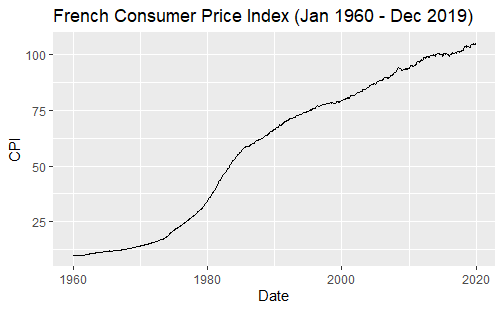
\includegraphics[width=\textwidth]{billeder/French_CPI_1960-2019.png}
        \caption{French CPI, 1960--2019}
        \label{fig:cpi}
    \end{minipage}
    \hfill
    \begin{minipage}{0.45\textwidth}
        \centering
        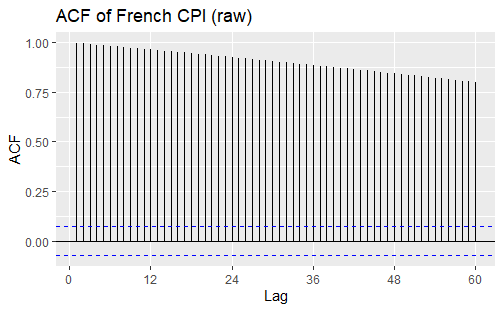
\includegraphics[width=\textwidth]{billeder/ACF_of_french_CPI_raw.png}
        \caption{Autocorrelation Function}
        \label{fig:acf}
    \end{minipage}
\end{figure}
The STL decomposition in Figure~\ref{fig:stl} isolates a smooth trend mirroring the raw series, a stable seasonal component ($\pm0.2$), and a small remainder with increased volatility around 2008--2009. A key limitation is that STL assumes an additive structure, whereas a multiplicative decomposition might be more appropriate given the growing trend with roughly constant seasonal amplitude.
\begin{figure}[H]
    \centering
    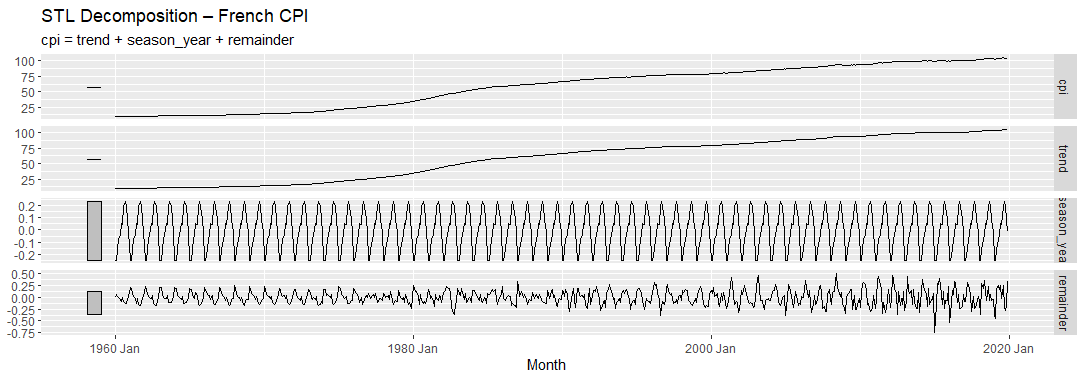
\includegraphics[width=1.0\textwidth]{billeder/STL_lille.png}
    \caption{STL Decomposition of French CPI}
    \label{fig:stl}
\end{figure}

%%%%%%%%%%%%%%%%%%%%%%%%%%%%%%%%%% Quesiton 1.2 %%%%%%%%%%%%%%%%%%%%%%%%%%%%%%%%%%

\section{Question 1.2}\label{Question 1.2}
Applying a natural log transformation to the CPI series does not fundamentally alter its 
properties. The series remains non-stationary with a strong upward trend, and the ACF in 
figure \ref{fig:acf_log} still decays very slowly, as in the original series.
\begin{figure}[H]
    \centering
    \begin{minipage}{0.45\textwidth}
        \centering
        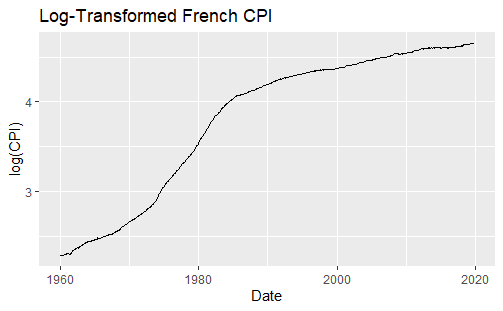
\includegraphics[width=\textwidth]{billeder/Log_transformed_French_CPI.png}
        \caption{Log-Transformed French CPI}
        \label{fig:log_cpi}
    \end{minipage}
    \hfill
    \begin{minipage}{0.45\textwidth}
        \centering
        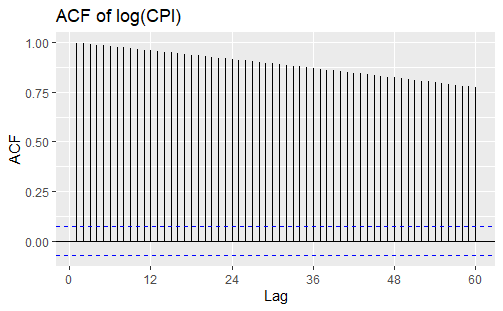
\includegraphics[width=\textwidth]{billeder/ACF_of_log_CPI.png}
        \caption{ACF – log(CPI)}
        \label{fig:acf_log}
    \end{minipage}
\end{figure}

The key difference is visible in the STL decomposition in figure \ref{fig:stl_log}: the seasonal component is now extremely small ($\pm0.004$) relative to the trend, and the remainder is much more homogeneous across the sample period, with no pronounced increase in volatility around 2008--2009. The Box-Cox procedure yields $\hat{\lambda} = 1.32$, which is close to 1, suggesting that little is gained from transforming the data. 

% We do however choose to work with the log-transformed series despite $\hat{\lambda} = 1.32$ being close to 1. When differenced, the original series exhibits non-constant variance that increases substantially from the 1970s onwards, violating a key ARIMA assumption. The log transformation stabilises this variance, making it suitable for ARIMA modelling.

We therefore choose to work with the original series for the remainder of the assignment, as neither the log transformation nor a power transformation is formally supported by the data, and the original CPI values are directly interpretable.

\begin{figure}[H]
    \centering
    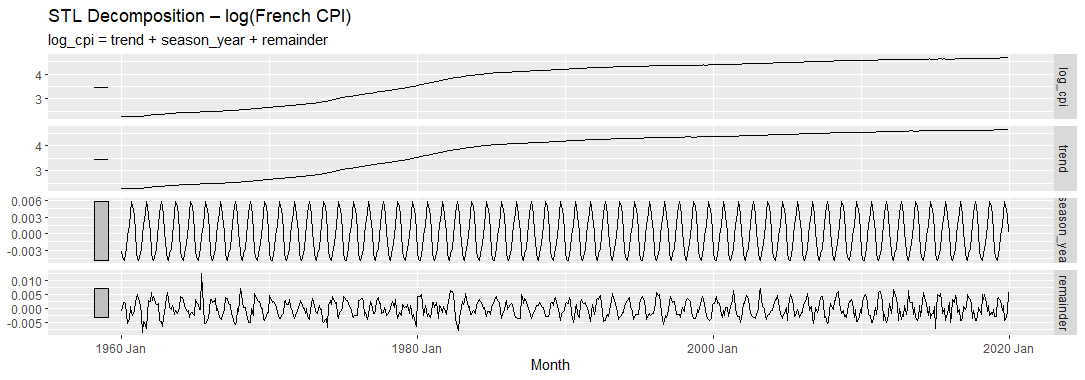
\includegraphics[width=1.0\textwidth]{billeder/log STIL lille.png}
    \caption{STL Decomposition – log(French CPI)}
    \label{fig:stl_log}
\end{figure}


%%%%%%%%%%%%%%%%%%%%%%%%%%%%%%%%%% Quesiton 1.3 %%%%%%%%%%%%%%%%%%%%%%%%%%%%%%%%%%

\section{Question 1.3} \label{Question 1.3}
Based on the analysis in question \ref{Question 1.1} and \ref{Question 1.2}, the CPI series exhibits a clear upward trend with no sign of mean reversion, indicating that the series is likely non-stationary. Both the ADF and KPSS tests are therefore applied in their standard specifications to formally verify this.

The ADF test yields a test statistic of $-0.761$ (p-value $= 0.965$), far above the 
5\% significance level, meaning we fail to reject the null hypothesis of a unit root. 
The KPSS test yields a statistic of $10.307$ (p-value $< 0.01$), strongly rejecting 
the null hypothesis of level stationarity. Both tests thus agree that the CPI series is non-stationary, consistent with the highly persistent ACF and the strong 
upward trend observed in question \ref{Question 1.1}.

%%%%%%%%%%%%%%%%%%%%%%%%%%%%%%%%%% Quesiton 1.4 gggfgsfgsgggggggggggggggggggggggggggggg
\section{Question 1.4} \label{Question 1.4}
The ADF and KPSS previusly reviel the need for furhter transformation. We will therefore transform the data by taking the difference. To determine the required order of differencing, we apply the KPSS-based unit root tests via \texttt{unitroot\_nsdiffs} and \texttt{unitroot\_ndiffs}. For both the original and log-transformed series, the tests indicate that one seasonal difference ($D = 1$) and one first-order difference ($d = 1$) are needed to achieve stationarity. We verify this by applying the ADF and KPSS tests to the differenced series: for both transformations, ADF rejects the unit root null ($p < 0.01$) and KPSS fails to reject the stationarity null ($p > 0.1$), confirming that the doubly differenced series are stationary.

To make the series stationary, we apply a seasonal difference (lag = 12) followed by a first-order difference. Figure \ref{fig:diff_cpi} shows the result for the original series: while trend and seasonality are removed, the variance is clearly non-constant, increasing substantially from the 1970s onwards. This confirms that the original series is inappropriate for ARIMA modelling despite $\hat{\lambda} = 1.32$ suggesting otherwise. We therefore proceed with the log-transformed series, whose differenced version in Figure \ref{fig:diff_log_cpi} exhibits a much more homogeneous variance throughout the sample period.

\begin{figure}[H]
    \centering
    \begin{minipage}{0.48\textwidth}
        \centering
        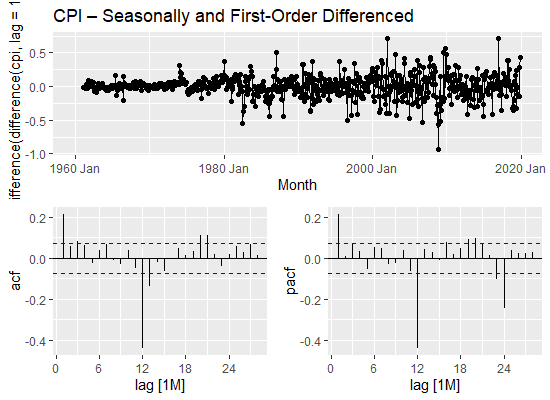
\includegraphics[width=\textwidth]{billeder/Seasonally_and_First-Order _differenced_lille.png}
        \caption{CPI – Seasonally and First-Order Differenced}
        \label{fig:diff_cpi}
    \end{minipage}
    \hfill
    \begin{minipage}{0.48\textwidth}
        \centering
        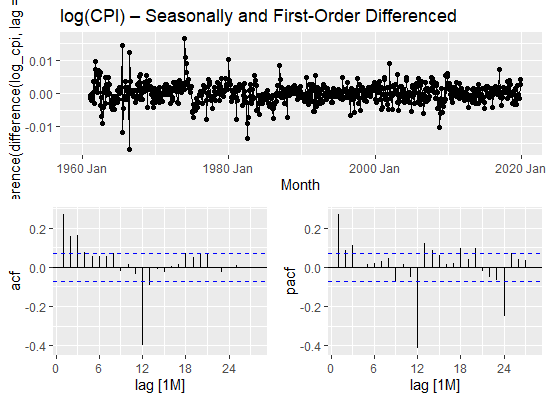
\includegraphics[width=\textwidth]{billeder/logcpi Seasonally and First-Order Dif- ferenced.png}
        \caption{log(CPI) – Seasonally and First-Order Differenced}
        \label{fig:diff_log_cpi}
    \end{minipage}
\end{figure}

Inspecting the ACF and PACF of the differenced log series, we observe a significant spike at lag 1 in the ACF that cuts off quickly, suggesting a MA(1) component ($q = 1$); a significant spike at lag 1 in the PACF, consistent with AR(1) ($p = 1$); and a large negative spike at lag 12 in both the ACF and PACF, indicating a seasonal MA(1) component ($Q = 1$). We therefore propose the following model:
\begin{equation}
    \text{ARIMA}(1,1,1)(0,1,1)_{12}
\end{equation}
where $d = 1$ reflects the first-order differencing, $D = 1$ the seasonal differencing with $m = 12$ months, $p = 1$ and $q = 1$ capture the non-seasonal AR and MA components, and $Q = 1$ captures the seasonal MA component.